In contrast to the previous project \cite{oldrepo}, no hardware design was provided. Therefore, the hardware design had to be created. The reference design \cite{TRDReferenceDesign} from Xilinx served as a template. It includes all the peripherals that are needed by the Linux kernel to run on the ZCU102 Evaluation Kit. The Vivado block design of the Zynq-related components can be seen in \cref{fig:hwzynq}.

\begin{figure}[htbp]
    \centering
    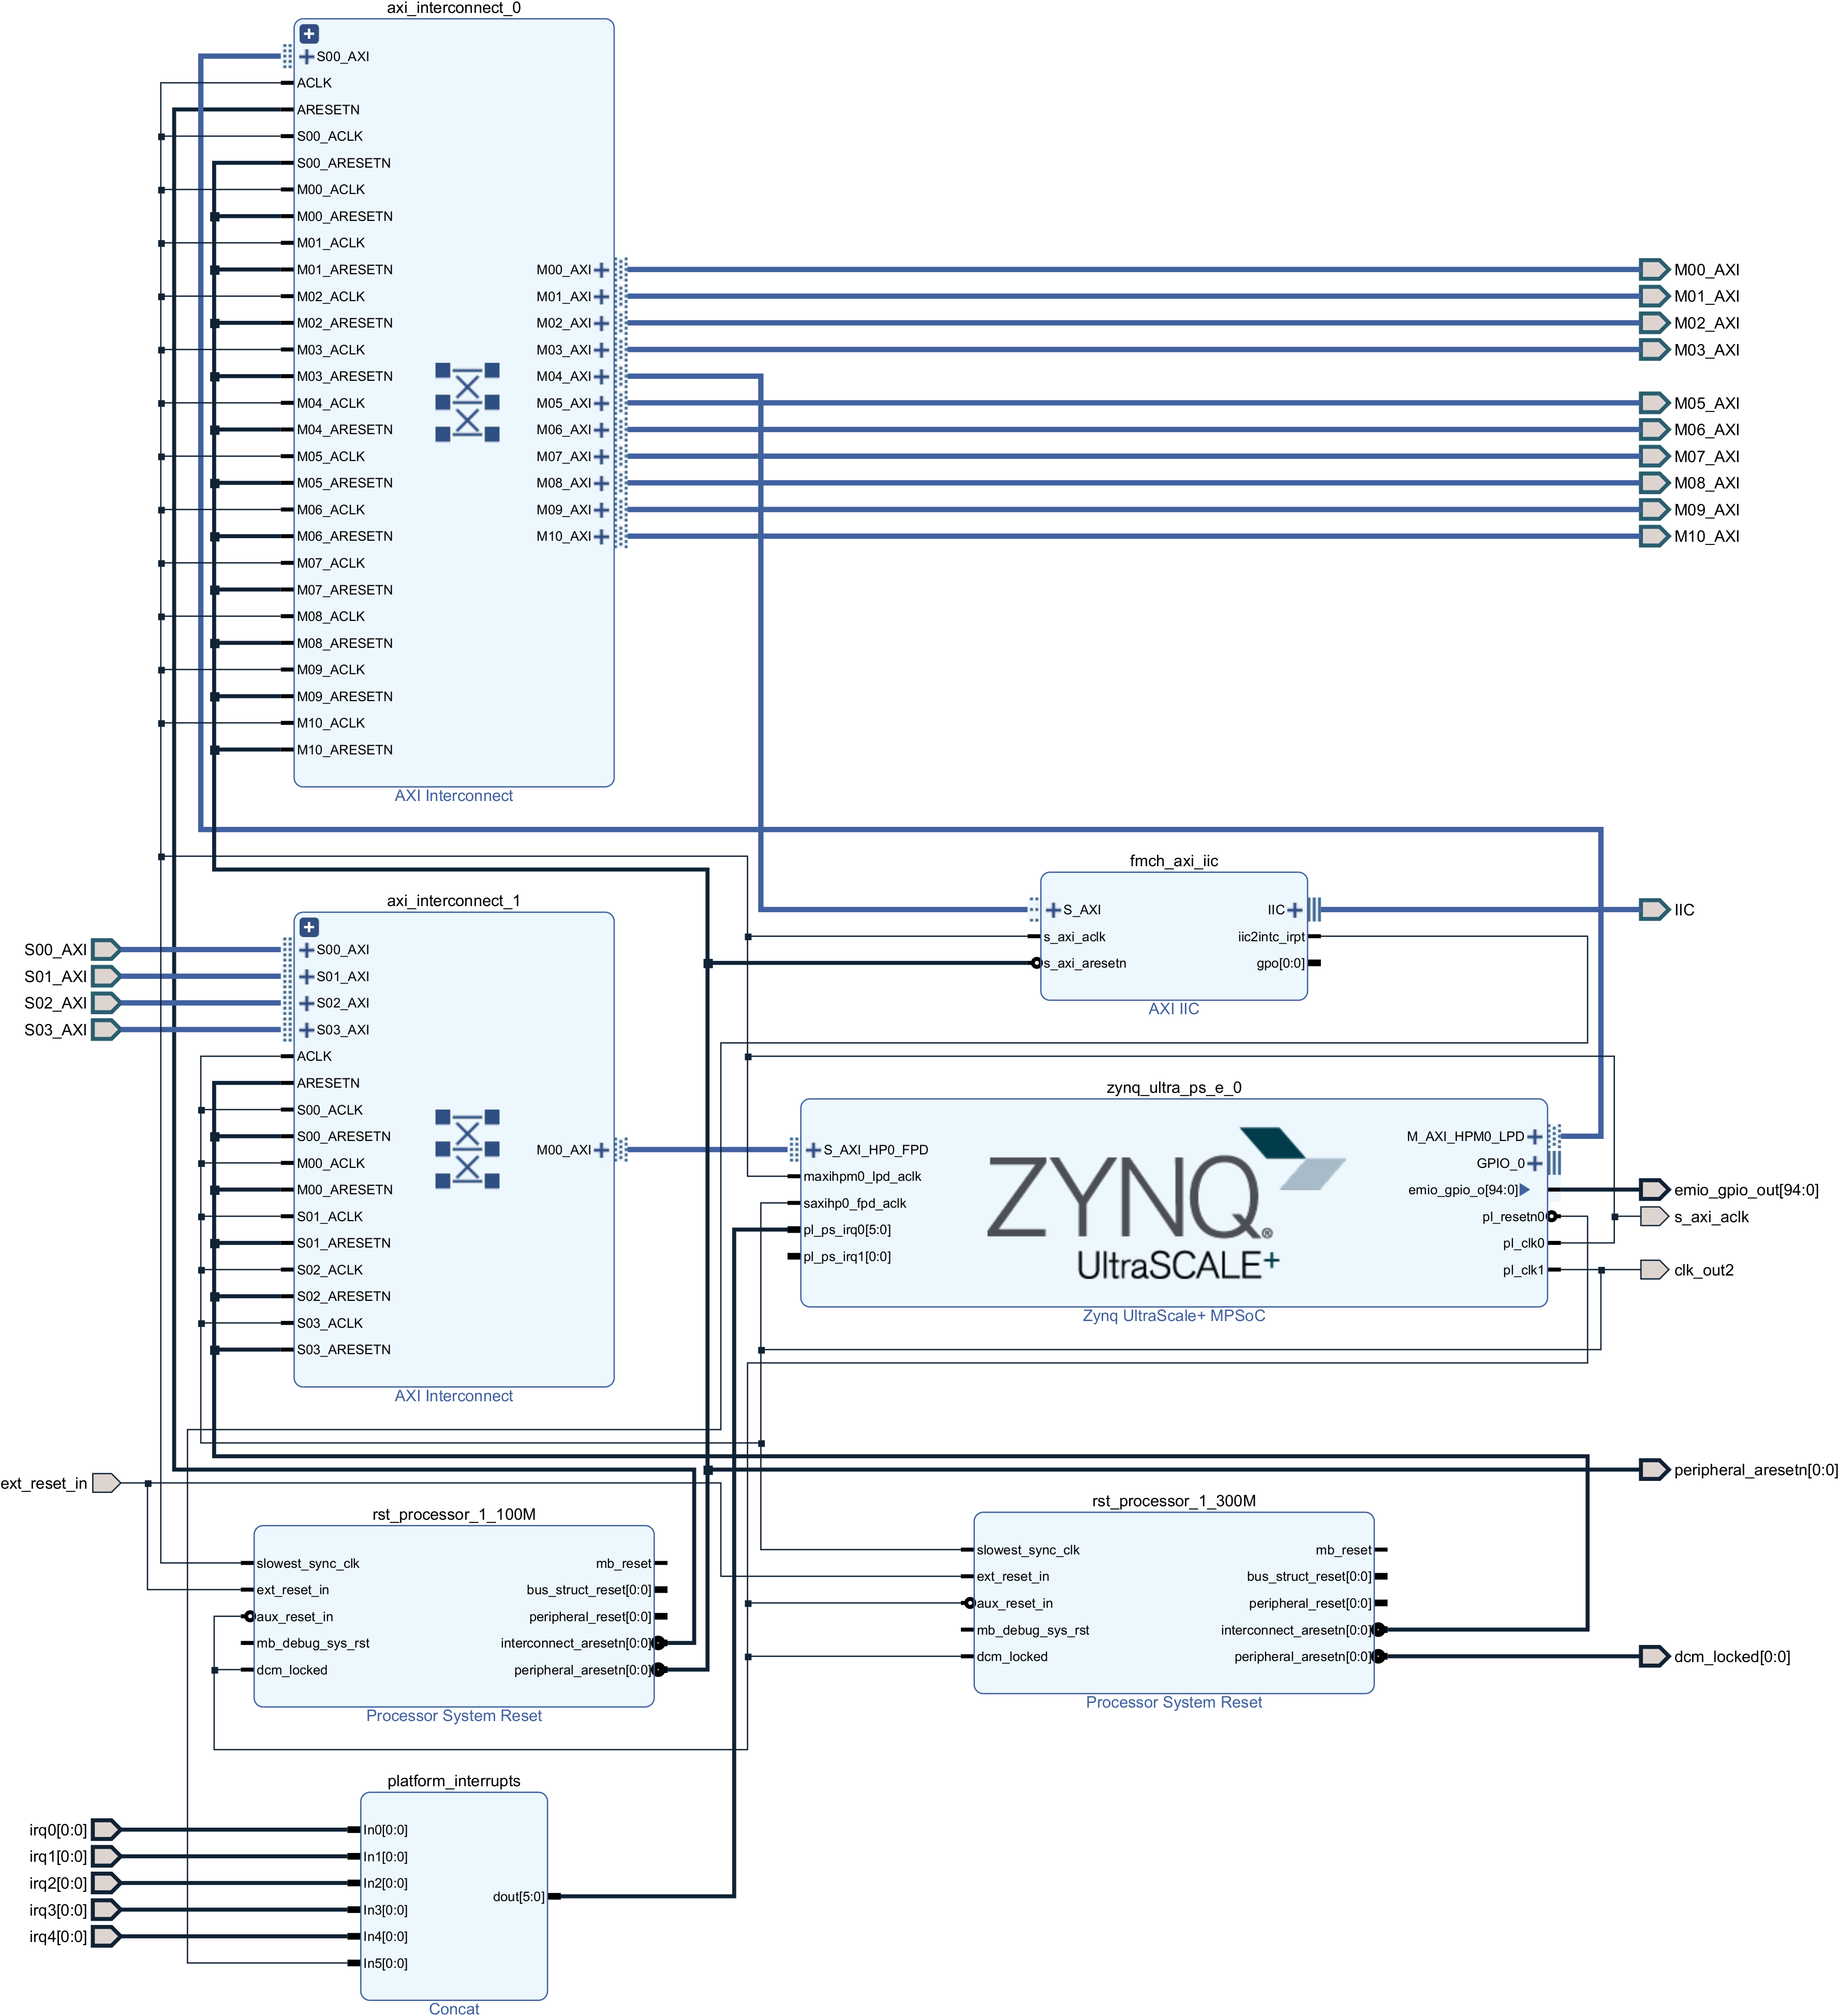
\includegraphics[width=1\textwidth]{images/hw-design-zynq.png}
    \caption{\label{fig:hwzynq} Vivado block design of Zynq-related components}
\end{figure}

This design is used to build the boot-image flashed onto the SD card that comes with the ZCU102 Evaluation Kit. It contains a Vivado block design project that can be opened and built using
the Xilinx Vivado Design Suite 2018.1.

This design can then be adapted to include our logic needed for the hardware accelerators. The Vivado IP packager flow described in \cite{UG1118} was used to include the custom hardware logic. Since the hardware accelerators were already created with the \gls{xps} tool included in the Xilinx ISE Design Suite, these hardware components only had to be repackaged as an \gls{ip} core for Vivado. The important thing is that you must complete these steps before enabling partial reconfiguration (see \cref{sssec:partialreconfigurationsetup}).
The basic steps to do this are:
\begin{itemize}
	\item Create new peripheral by choosing `Tools', `Create and Package New IP\ldots'
	\item Select `Package a specified directory' as package option
	\item The new peripheral can now be found in the `IP Catalog'
		under the `User repository'.
		Add it to the design by double clicking on it and choosing `Add IP to Block Design'
	\item Connect the \gls{ip} core to the Zynq Processing System
	\item Assign an address and memory size in the `Address Editor' tab
\end{itemize}
For the last step, choose a free address.
The custom logic cores can be assigned addresses starting from $0x88000000$ in the address-table.

Each \gls{ip} core from the previous project contains two main \gls{vhdl} files.
One is called `user\_logic.vhd' and the other carries the name of the core
itself.
The first one contains the actual logic and a simple interface so that the logic can react to register reads and writes.
The second file maps that simple interface to the \gls{axi} interface so that it can be connected to Zynq's \gls{axi} bus.

The complete hardware design can be generated running the following commands in the git repository at \emph{<repo>/hardware\_design/}:

\begin{lstlisting}[
	language=Bash,
	%caption={Synthesis for project},
	%label={lst:makehwdesign},
	basicstyle=\small,
	float=htbp,
	floatplacement=htbp
	]
# if the hardware design has not yet been created, run ...
make -f scripts/Makefile create
# generate the hardware design and the bitstreams
make -f scripts/Makefile bit
\end{lstlisting}
\FloatBarrier

The logic design of the two hardware accelerators is discussed in the following
subsections.
